% THIS TEMPLATE IS A WORK IN PROGRESS
% Adapted from an original template by faculty at Reykjavik University, Iceland

\documentclass{scrartcl}

% Adapted from an original template by Hlyni Arnórssyni, Reykjavik University, Iceland
%
% ------------------------------ SETTINGS
\usepackage{geometry}

\geometry{
	paper=a4paper, % Paper size
	top=2.5cm, % Top margin
	bottom=2.5cm, % Bottom margin
	left=2.5cm, % Left margin
	right=2.4cm, % Right margin
	headheight=0.75cm, % Header height
	footskip=1.5cm, % Space from the bottom margin to the baseline of the footer
	headsep=0.75cm, % Space from the top margin to the baseline of the header
	%showframe, % Uncomment to show how the type block is set on the page
}

\usepackage{blindtext}
%-------------------------------- Character encoding ----------------------------
\usepackage[T1]{fontenc}
\usepackage[utf8]{inputenc}

%----------------------------- Mathematics packages from AMS ---------------

\usepackage{amsmath, amsfonts, amsthm, amssymb}
\usepackage{braket, nicefrac}

% ----------- International System of Units
\usepackage{siunitx}

%------------------------------ Lists / numbers -------------------------
\usepackage{enumitem, multicol}

%------------------------------- Figure insertions --------------
\usepackage{graphicx, float}  % Use option [H] to force the placement of a figure
\usepackage{keystroke}
\usepackage{pgfplots}\usepgfplotslibrary{units}\pgfplotsset{compat=1.16}

%------------------------------- Line Spacing --------------
\usepackage{setspace}

%------------------------------- Depth of the ToC --------------
\setcounter{tocdepth}{2}

%%%%%%%%%%%%%%%%%%%%%%%%%% Hyperlink References %%%%%%%%%%%%%%%%%%%%%%%%%%%
\usepackage{hyperref}

%--------------------% Storage Path for images %-----------------%
\graphicspath{{graphics/}{Graphics/}{./}{./research-paper/capstone/capstone/Graphics}}

%%%%%%%%%%%%%%%%%%%%%%%%%% Environments %%%%%%%%%%%%%%%%%%%%%%%%%%%
\renewenvironment{abstract}{
    \begin{center}
    \textbf{Abstract}
    \vspace{0.5cm}
    \par\itshape
    \begin{minipage}{0.8\linewidth}}{\end{minipage}
    \noindent\ignorespaces
    \end{center}
}

\newenvironment{keywords}{
    \begin{center}
    \textbf{Keywords}
    \vspace{0.5cm}
    \par
    \begin{minipage}{0.8\linewidth}}{\end{minipage}
    \noindent\ignorespaces
    \end{center}
}

\newenvironment{preface}{
    \begin{center}
    \textbf{Preface}
    \vspace{0.5cm}
    \par
    \begin{minipage}{0.8\linewidth}}{\end{minipage}
    \noindent\ignorespaces
    \end{center}
}

\newenvironment{acknowledgements}{
    \begin{center}
    \textbf{Acknowledgements}
    \vspace{0.5cm}
    \par
    \begin{minipage}{0.8\linewidth}}{\end{minipage}
    \noindent\ignorespaces
    \end{center}
}

\hbadness=10000

\begin{document}
%Title of the report, name of coworkers and dates (of experiment and of report).
\begin{titlepage}
	\centering
	
\includegraphics[width=0.6\textwidth]{nyush-logo.jpeg}\par
	\vspace{2cm}
	%%%% COMMENT OUT irrelevant lines among the 3 below
  {\scshape\LARGE Computer Science, Data Science \& \par}  %if you're a CS major
  {\scshape\LARGE Computer Systems Engineering \par}
	\vspace{1cm}
	{\scshape\Large Capstone Report - Fall 2024\par}
	%{\large \today\par}
	\vfill
	
	%%%% PROJECT TITLE
	{\huge\bfseries Benchmarking ZK Virtual Machines for Privacy-Preserving Machine Learning Applications\par}
	\vfill
	
	%%%% AUTHOR(S)
	{\Large\itshape Lawrence Lim\\ Siddhartha Tuladhar\\ Brandon Gao\\}\par
	\vspace{1.5cm}

	\vfill
	supervised by\par
	%%%% SUPERVISOR(S)
  Promethee Spathis

	\vfill
% Bottom of the page
\end{titlepage}

\newpage

\begin{preface}
 As a team comprising a Computer Systems Engineering major, a Computer Science major, and a Data Science major, we bring diverse perspectives and expertise to address the complex challenges at the intersection of privacy, security, and scalability in technology. This project was inspired by the increasing importance of privacy-preserving computation, particularly in sensitive fields like finance, where secure data handling is paramount. Our collective academic backgrounds have allowed us to explore innovative approaches to these challenges, drawing from distributed systems, cryptography, and data analytics.

Our target audience includes researchers, developers, and industry professionals who are advancing privacy technologies, blockchain systems, and secure data frameworks. By benchmarking zero-knowledge virtual machines (zkVMs) in the context of financial data, this project seeks to provide valuable insights into their capabilities and limitations, contributing to the ongoing development of secure and privacy-centric computational tools.       
\end{preface}

\vspace{1cm}

\begin{acknowledgements}
We sincerely thank our advisor, Professor Promethee Spathis, for their guidance and support throughout this project. We are also grateful to the Professor Benedikt Bunz for providing the initial ideation for this project. Lastly, we are grateful to our families and friends for their encouragement and support.\end{acknowledgements}

\newpage

\begin{abstract}
This work addresses the challenge of securely processing sensitive data in privacy-critical applications like finance. Zero-knowledge virtual machines (zkVMs) offer a promising solution, but face issues with complexity and proof generation time. We benchmark three zkVMs—SP1, Jolt, and RISC-0—by training a ridge regression model on financial data, evaluating their performance and identifying key bottlenecks. Our findings highlight zkVMs’ potential for privacy-preserving computation and provide insights for improving their practical adoption.
\end{abstract}
\vspace{1cm}

\begin{keywords}
\centering
         \textbf{Capstone; Computer science; Machine Learning; Zero-Knowledge Proofs, Zero-Knowledge Virtual Machines, Jolt, SP1, Risc0, NYU Shanghai}
\end{keywords}

\newpage



\doublespacing
\tableofcontents
\singlespacing

\newpage

\doublespacing

\section{Introduction}

\subsection{Context}

Currently, there exists a large amount of sensitive customer data that is extremely valuable but not being monetized to its fullest extent due to a combination of compliance and ethical concerns. An essential category of this data is personal financial data. Due to the sensitive nature of this data and strict compliance laws, current Fintech platforms require users’ explicit permission to access sensitive information like credit history, transaction history, and income. However, \textbf{Zero Knowledge Proof (ZKP)} can be utilized to develop services and algorithms that utilize the sensitive data without explicitly revealing it. A ZKP is a cryptographic method of proving a statement is true without revealing any other information besides the fact that the statement is true. ZKPs have three fundamental characteristics:

\begin{itemize}
    \item \textbf{Completeness:} If a statement is true, an honest prover can prove to an honest verifier that they have knowledge of the correct input.
    \item \textbf{Soundness:} If a statement is false, a dishonest prover is unable to convince an honest verifier that they have knowledge of the correct input.
    \item \textbf{Zero-knowledge:} No other information about the input is revealed to the verifier from the prover besides the fact that the statement is true.
\end{itemize}

Currently, the most-friendly way of generating a ZKP is through the use of zero-knowledge virtual machines (zkVMs). A zkVM, is simply a VM implemented as a circuit for a ZKP system. So, instead of proving the execution of a program, as one would normally do in ZKP systems, you prove the execution of the bytecode of a given Instruction Set Architecture (ISA). However, the zkVM landscape is in early development, and proof generation is bottlenecked by the complexity of the program and hardware limitations. In this paper, we provide a quantatitve and qualitative analysis on the current state of zkVMs on a real-world use case by generating a proof of a machine learning (ML) algorithm on dummy financial data.

\subsection{Objective}

The objective of this paper is to provide researchers, developers, and industry professionals a comprehensive review on utilizing zkVMs in a real-world use case. In order to achieve this, we benchmark SP1\cite{Roy2024}, Risc0\cite{bruestle2023risc}, and Jolt\cite{arun2024jolt}, since they all compile to RISC-V, which is an extremely popular compile target for most programming languages (Rust, C++, LLVM). We provide a quantative analysis on proof generation time and proof verification time. Additionally, we provide a qualitative analysis on the developer experience on developing ML algorithms for these zkVMs. The ML algorithm that we use is the ridge regression model. 

\section{Related Work}

%%%% DO NOT write a related work section that is just a laundry list of other papers, with a sentence about each one that was lifted from its abstract, and without any critical analysis nor deep comparison to other work.

\subsection{Virtual Machine-based ZK Systems}

 Our research explores the most efficient methods for generating ZKPs for machine learning algorithms by experimenting with different zkVMs. The current papers on zkVMs focus on their architecture and the techniques that are used by the zkVM to achieve optimized proof and verification times. For example, Arun et al.\cite{arun2024jolt} present Jolt, a zero-knowledge Succinct Non-Interactive Argument of Knowledge (zkSNARK) system optimized for VMs, which uses a new lookup technique to reduce proof size and verification time. Their paper focuses on this optimization that makes Jolt effective in environments where complex computations occur, and proof generation must remain efficient. Similarly, Bruestle and Gafni\cite{bruestle2023risc} introduce RISC-0, a system designed to produce scalable, transparent proofs for computations based on the RISC-V instruction set. RISC-0 focuses on architecture-specific applications, such as the RISC-V ecosystem, which contrasts with Jolt’s broader application to virtual machines. Currently, there is no literature on the direct comparison between these zkVMs, which is the objective of our paper. Additionally, there is no research or comparisons on SP1. 

\subsection{Machine Learning in ZKPs}

Machine learning is a highly relevant use case for ZKPs. There are multiple articles on the various use cases of ML in ZKPs. Wang et al.\cite{wang2024efficient} developed an efficient ZKP-based pipeline for classical machine learning inference, focusing on privacy-preserving inference that ensures model accuracy without exposing sensitive model information. This system optimizes zero-knowledge inference, making it highly applicable to real-world ML applications where data privacy is paramount. Our paper uses the same inference technique within the zkVM as a real world application. Similarly, Sathe et al.\cite{sathe2024survey} provide a comprehensive survey of ZKP applications in machine learning, covering a range of cryptographic techniques and their applicability to neural networks, decision trees, and other ML models. Their survey offers a broader comparison of ZKP techniques in the ML space, providing essential context for more specific systems like that of Wang et al. However, their paper does not provide details on the performance or real-world use case. Lastly, Ganescu and Passerat-Palmbach\cite{ganescu2024trust} extend the application of ZKPs to generative AI models, by proposing a system that enhances trust in AI by allowing for the verification of generative models without exposing underlying data, which is critical in AI-driven environments where sensitive inputs and outputs must be safeguarded while still proving the model’s validity. This paper is similar to Wang et al., where it provides a real-world use case, but it utilizes generating ZKPs through tools that are inaccessible to developers and require high development overhead. By using zkVMs, most of the ZKP logic is abstracted away, which provides developers easier access to converting their programs into ZKPs.

\section{Solution}

The methodology for achieving our objective is structured into two key phases. The first phase involves developing and training a machine learning algorithm on a given dataset to attain satisfactory accuracy levels. The second phase entails exporting the trained model and test data into Rust, where the inference process is meticulously implemented by manually translating the logic from Python to Rust.


\subsection{Data Preparation}
In this study, we aimed to predict customer spending for the next 90-day period (i.e., the last quarter) based on historical transaction data. The methodology consists of several key steps, including data preprocessing, feature engineering, model training, and evaluation. Below, we detail each step of the process.

The dataset comprises customer transactions, with each record containing information on the transaction date, product price, quantity purchased, and customer ID. The first step in the data preparation process involved determining a cutoff date that would separate the historical data used for training from the future data we wish to predict. We defined this cutoff date as 90 days before the latest transaction in the dataset. This allowed us to segment the data into two parts:

\begin{itemize}
    \item \textbf{Training Data (First Three Quarters):} Transactions occurring before the cutoff date, which we used to derive customer behavior features (recency, frequency, and monetary values).
    \item \textbf{Target Data (Fourth Quarter):} Transactions occurring after the cutoff date, which were used to calculate the target variable, customer spending in the last quarter (\texttt{actual\_spend\_90\_days}).
\end{itemize}

To align the data with fiscal years, we defined the quarters as follows:

\begin{itemize}
    \item \textbf{Q1 (Fiscal):} April 29 -- July 31, 2023
    \item \textbf{Q2 (Fiscal):} August 1 -- October 31, 2023
    \item \textbf{Q3 (Fiscal):} November 1, 2023 -- January 31, 2024
    \item \textbf{Q4 (Fiscal):} February 1 -- April 28, 2024
\end{itemize}

These fiscal quarters allow us to capture patterns that could impact customer spending. For example, Q1 includes spring and early summer, while Q4 spans the winter and early spring periods.

We used these defined fiscal quarters to organize the data, aggregating customer spending within each quarter to track how spending evolves over time. The ultimate goal was to use the data from Q1, Q2, and Q3 to predict customer spending in Q4.

\subsection{ML Setup}

In order to simulate real-world transaction data, dummy transaction data was taken from a Kaggle dataset\cite{rehman2023retail}. The dataset was processed to extract key features such as recency, frequency, monetary value (RFM), and spending activity, which is depicted in Table \ref{tab:dataset_description}. RFM serves as a foundation for predictive modeling, where these metrics can be combined with other features to enhance the accuracy of customer spending predictions. 


\begin{table}[ht!]
\centering
\begin{tabular}{|l|p{10cm}|}
\hline
\textbf{Field} & \textbf{Description} \\
\hline
\textbf{CustomerID} & Unique identifier for a customer, used to track and differentiate individuals in the dataset. \\
\hline
\textbf{Frequency} & Number of transactions a customer made during the first three quarters. \\
\hline
\textbf{Monetary} & Total monetary value of a customer's transactions during the first three quarters. \\
\hline
\textbf{Recency} & Number of days since the customer's last transaction during the first three quarters. \\
\hline
\textbf{Price} & Price per unit for each transaction item. \\
\hline
\textbf{DiscountApplied} & Percentage of discount applied to the transaction. \\
\hline
\textbf{spend\_90\_flag} & Binary flag indicating whether the customer made any transaction in the past 90 days. \\
\hline
\textbf{actual\_spend\_90\_days} & Total amount spent by the customer in the last 90 days(quarter). \\
\hline
\end{tabular}
\caption{Description of fields in the customer transaction dataset.}
\label{tab:dataset_description}
\end{table}

For the machine learning algorithm, we used the Ridge Regression Model due to the model's accuracy and the complexity constraints of the zkVMs. Ridge Regression is an extension of linear regression by adding a penalty term to the loss function to prevent overfitting.  Ridge Regression prevents overfitting by penalizing large coefficient values, thereby shrinking them towards zero. The Ridge Regression loss function is formulated as:
\[
\text{Loss} = \sum_{i=1}^{m} \left( y_i - \hat{y}_i \right)^2 + \lambda \sum_{j=1}^{n} w_j^2
\]
where \( m \) is the number of samples, \( n \) is the number of features, \( \hat{y}_i \) represents the predicted value for the \( i \)-th sample, \( \lambda \) is the regularization parameter controlling the strength of the penalty, and \( w_j \) are the model coefficients. The second term \( \lambda \sum_{j=1}^{n} w_j^2 \) is the regularization term, which discourages large coefficients and helps reduce the model's variance. The accuracy of the model is shown in Table \ref{tab:model-performance}.

\begin{table}[h!]
\centering
\begin{tabular}{|l|c|p{8cm}|}
\hline
\textbf{Metric} & \textbf{Value} \\
\hline
\( R^2 \)(R-Squared) & 0.8  \\
\hline
Mean Square Error (MSE) & 21 \\
\hline
\end{tabular}
\caption{Model performance metrics.}
\label{tab:model-performance}
\end{table}

The \(R^2\) value measures the proportion of variance in the target variable that is explained by the independent variables in the model. It ranges from 0 to 1, where higher values indicate a better fit of the model to the data.

The MSE represents the average squared difference between the predicted and actual values. It provides a measure of the model's prediction error, with lower values indicating better performance.

\subsection{zkVM Implementation}

The zkVM implementation for all three included exporting the model (as a JSON file) and inference dataset. The inference dataset was parsed, 
\begin{figure}[H]
	\begin{center}
		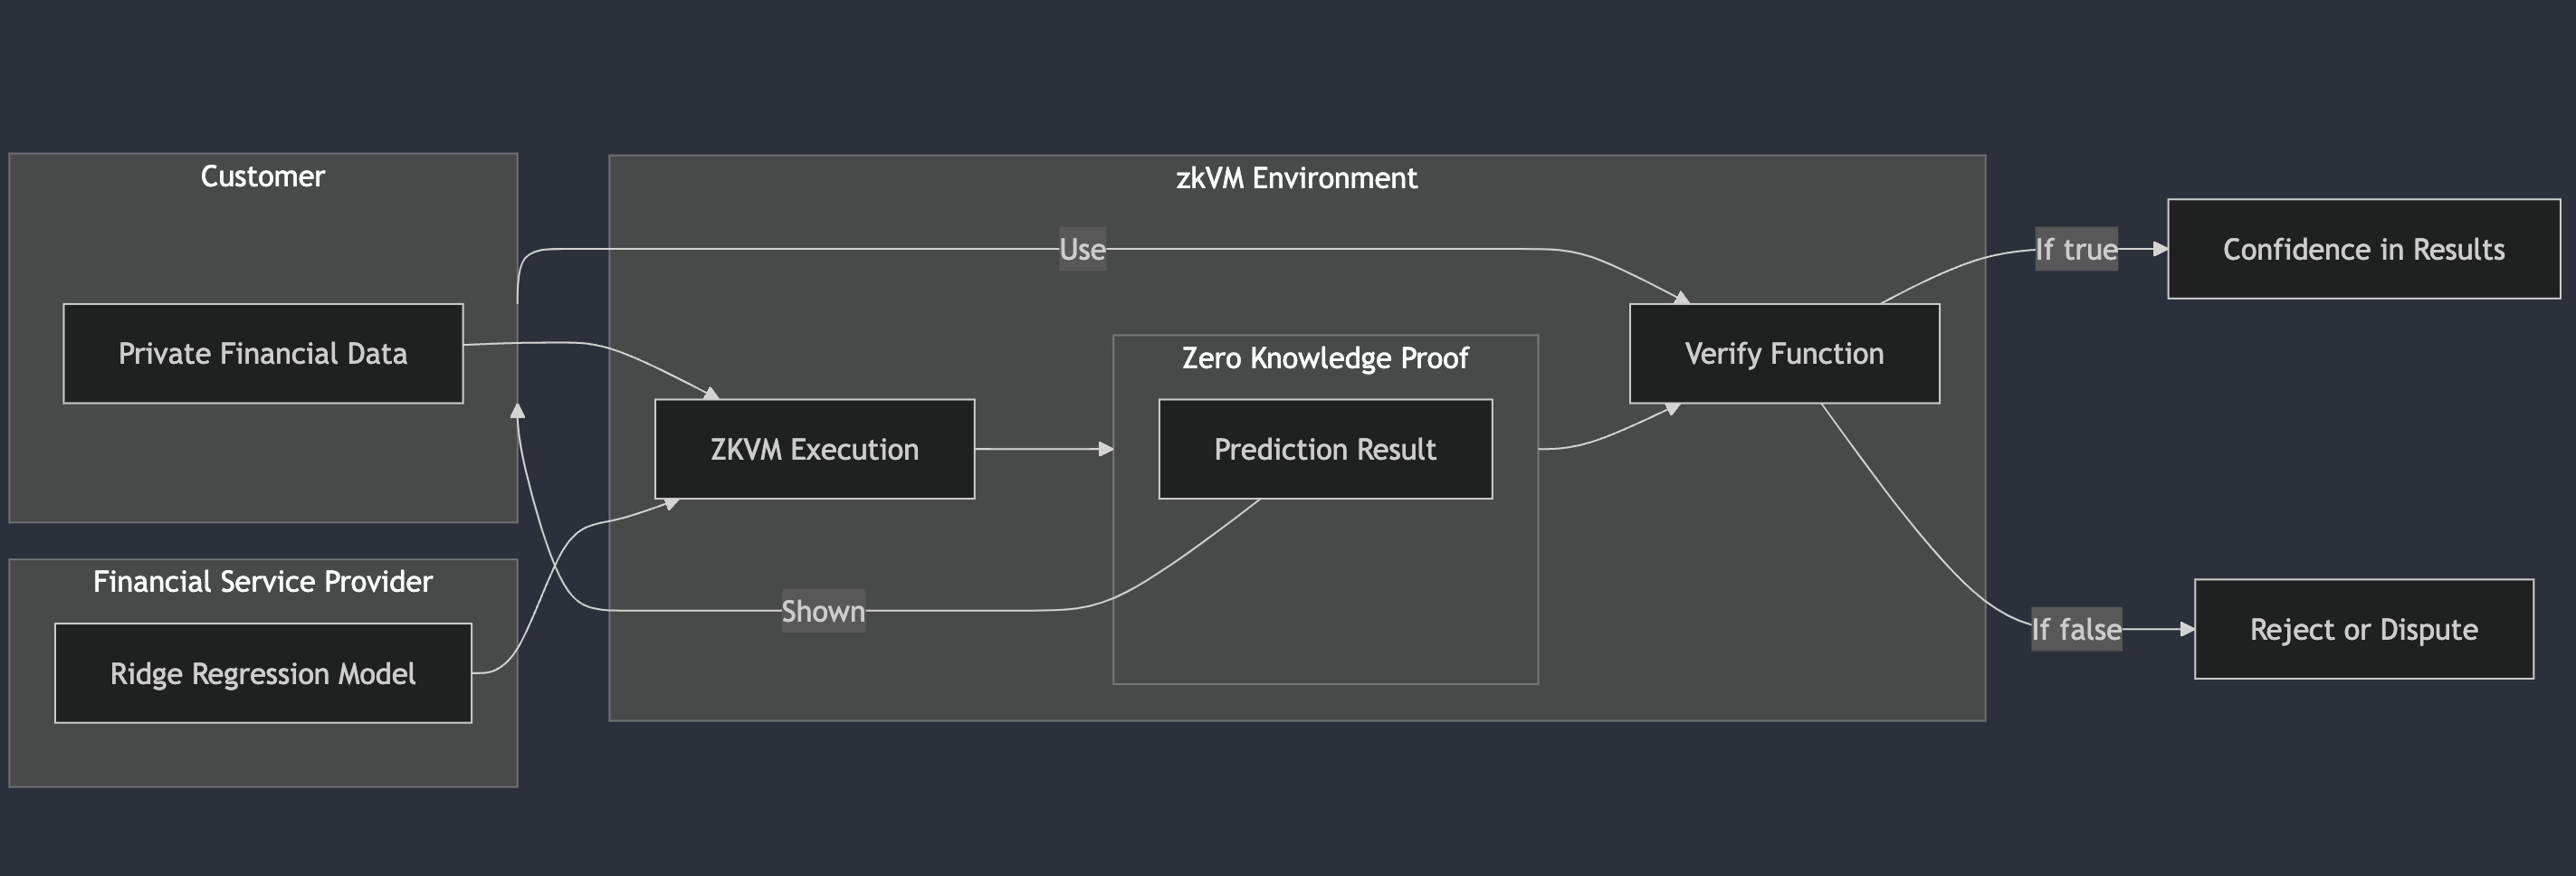
\includegraphics[scale=0.35]{zkVM-design.png}
	\end{center}
	\caption{Architecture of our benchmark procedure}
	\label{fig:architecture}
\end{figure}

\section{Results}

The results section details your metrics and experiments for the assessment of your solution. It then provides experimental validation for your approach with visual aids such as data tables and graphs. In particular, it allows you to compare your idea with other approaches you've tested, for example solutions you've mentioned in your related work section.

% \subsection{Data tables}
%
% Every data table should be numbered, have a brief description as its title, and specify the units used. 
%
% As an example, Table compares the average latencies of native application calls to networked services. The experiments were conducted on an Apple MacBook Air 2010 with a CPU speed of 1.4GHz and a bus speed of 800MHz. Each data point is a mean over 20 instances of each call, after discarding both the lowest and the highest measurement.
%
% \subsection{Graphs}
%
% Graphs are often the most important information in your report; you should design and plot them with great care. A graph contains a lot of information in a short space. Graphs should be numbered and have a title. Their axes should be labelled, with the quantities and units specified. Make sure that individual data points (your measurements) stand out clearly. And of course, always associate your graph with text that explains your results, and outlines the conclusions you draw from these results.
%
\subsection{ARM Benchmark}

\begin{figure}
	\begin{center}
		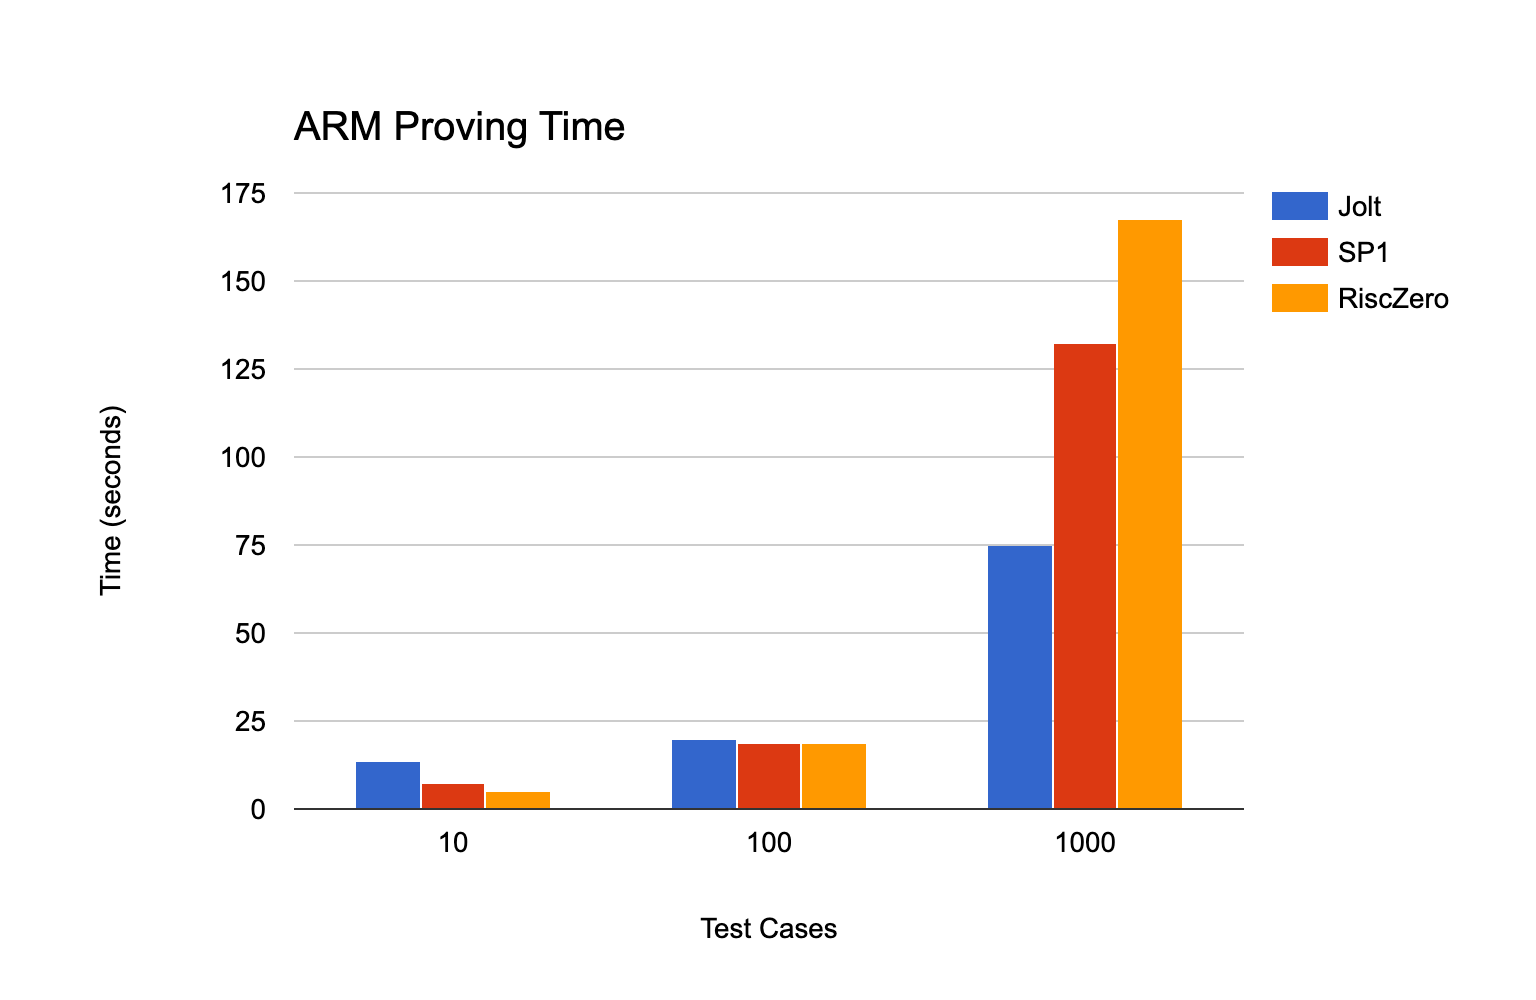
\includegraphics[width=\linewidth]{ARM-Proving-Time.png}
	\end{center}
	\caption{ARM Proving Time}
	\label{graph:arm-proving-time}
\end{figure}

For example, Figure~\ref{graph:arm-proving-time} compares the efficiency of three different service architectures in eliminating adversarial behaviors. Every data point gives the probability that $k$ faulty/malicious nodes managed to participate in a computation that involves 32 nodes. In the absence of at least one reliable node ($k = 32$), the failure will go undetected ; but the results show that this case is extremely unlikely, regardless of the architecture. The most significant result pertains to $k = 16$: the reliable nodes detect the failure, but cannot reach a majority to recover. The graph shows that the \texttt{CORPS 5\%} architecture is much more resilient than the \texttt{DHT 30\%} architecture, by a magnitude of $10^{11}$.

\begin{figure}
	\begin{center}
		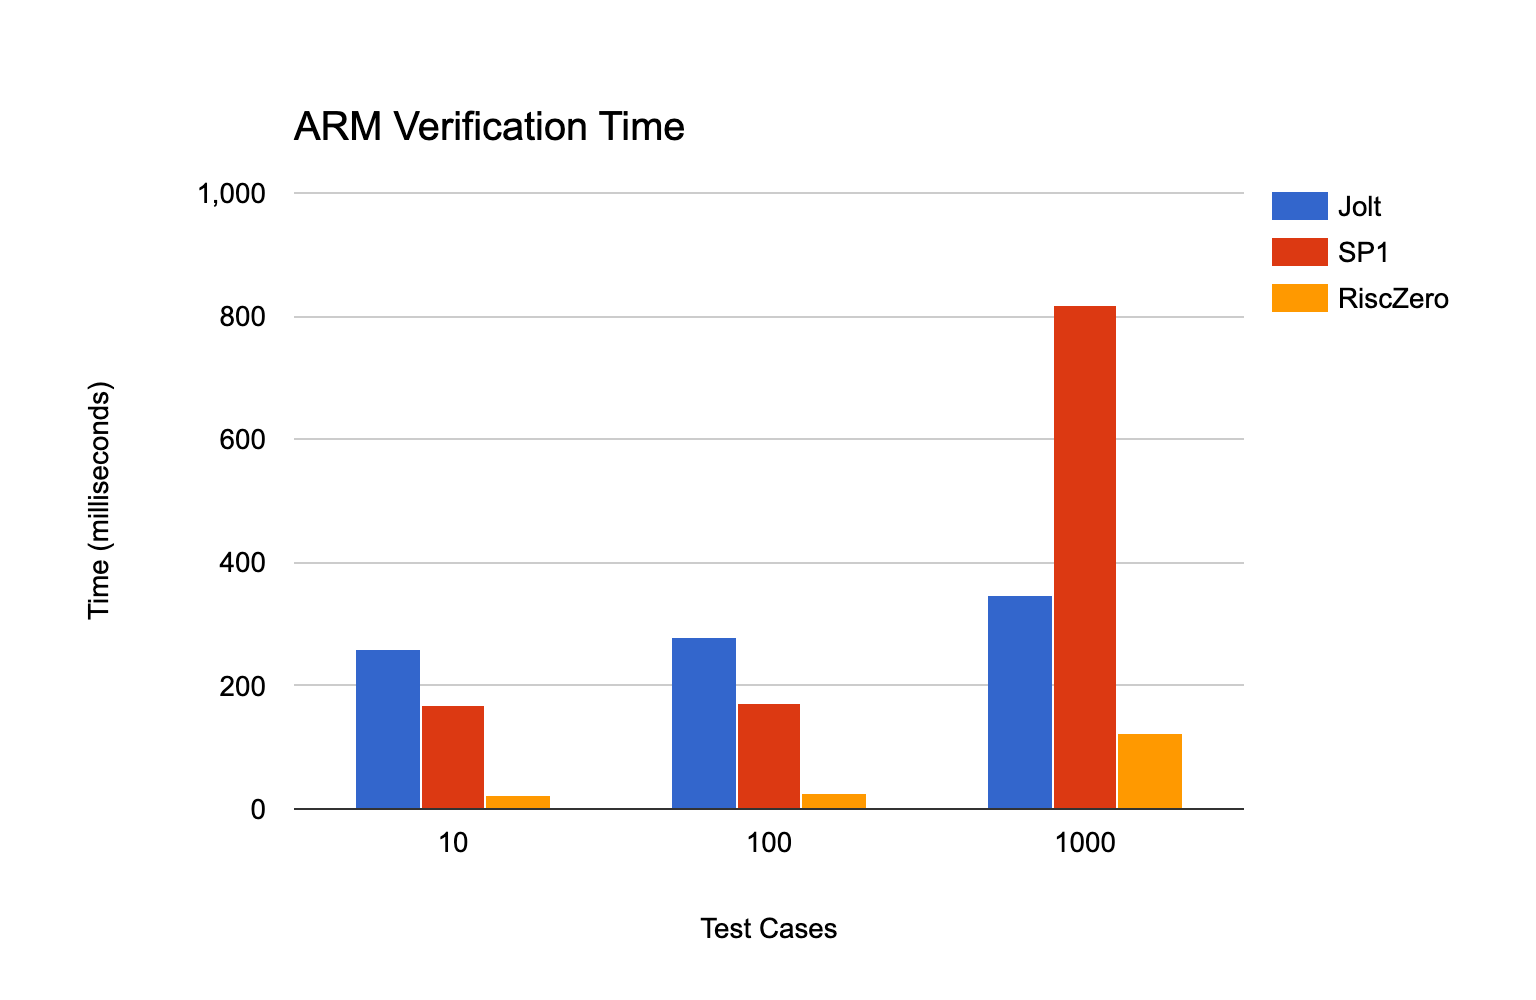
\includegraphics[width=\linewidth]{ARM-Verification-Time.png}
	\end{center}
	\caption{ARM Verification Time}
	\label{graph:arm-verification-time}
\end{figure}

\subsection{x86 Benchmark}

\begin{figure}
	\begin{center}
		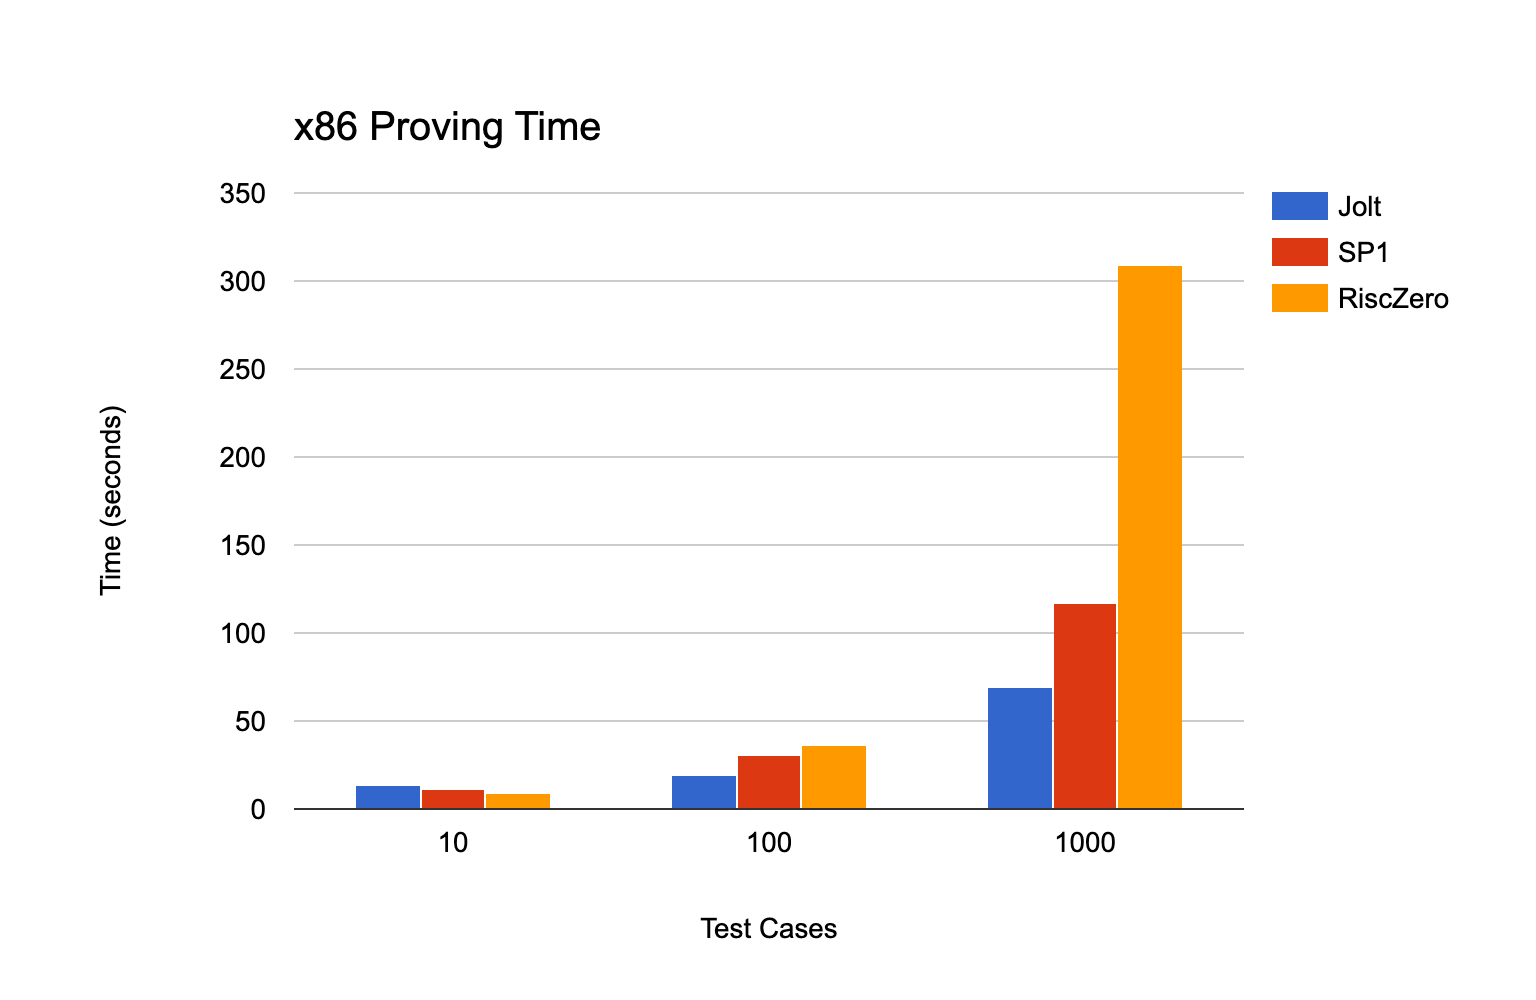
\includegraphics[width=\linewidth]{x86-Proving-Time.png}
	\end{center}
	\caption{x86 Proving Time}
	\label{graph:x86-proving-time}
\end{figure}

\begin{figure}
	\begin{center}
		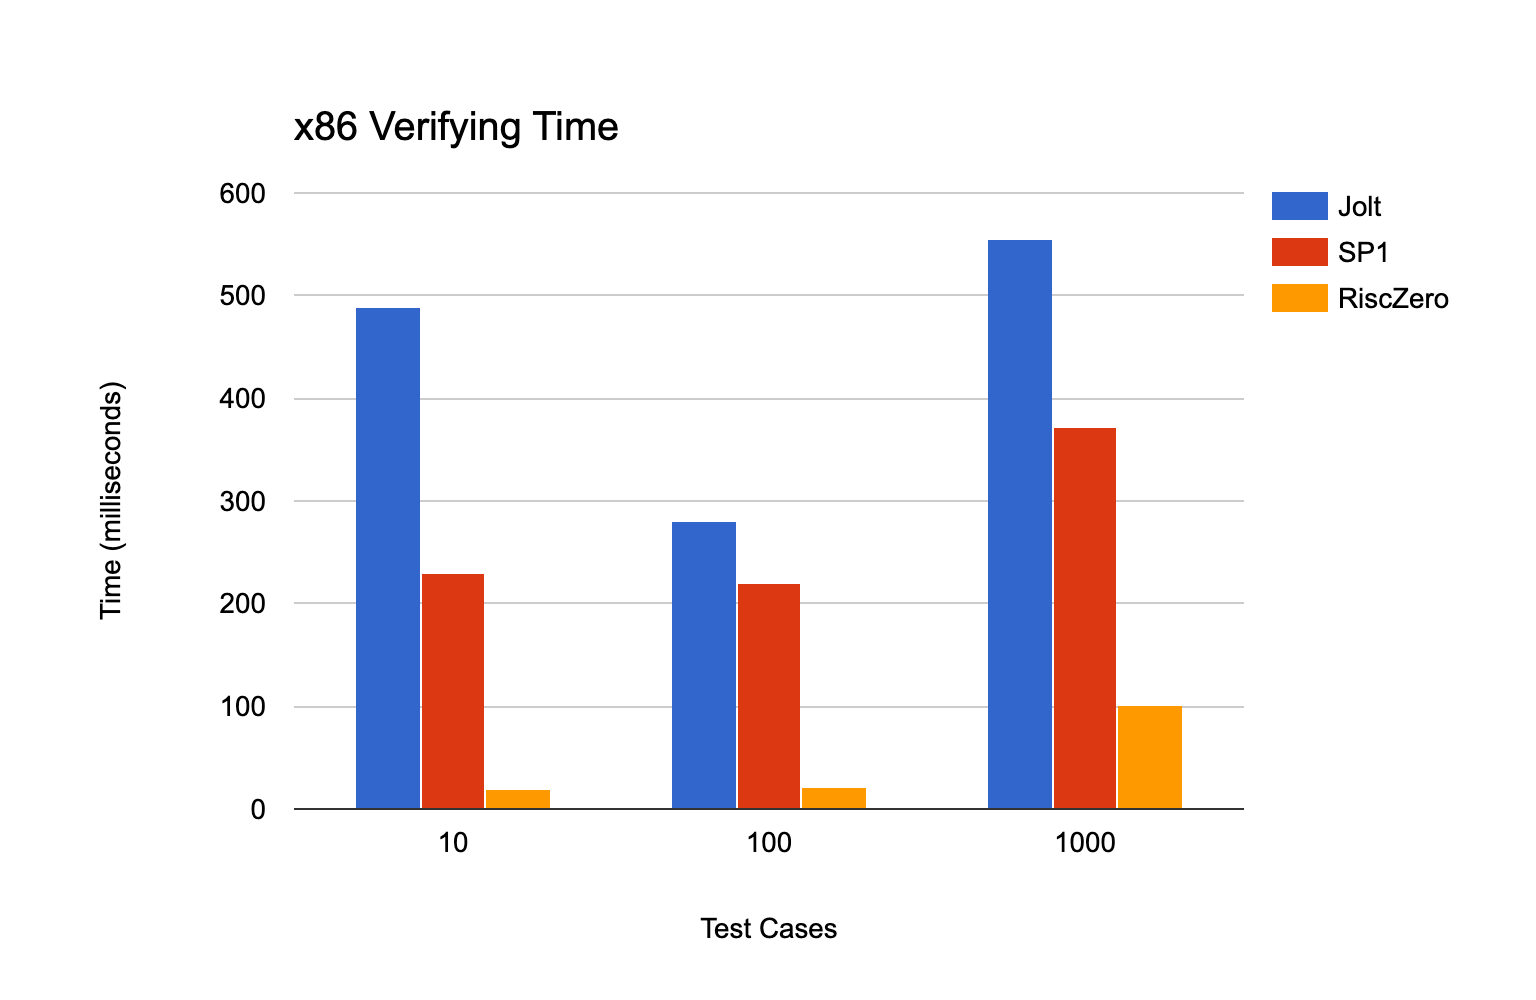
\includegraphics[width=\linewidth]{x86-Verification-Time.png}
	\end{center}
	\caption{x86 Verification Time}
	\label{graph:x86-verification-time}
\end{figure}

\subsection{Performance Metrics}


\subsection*{Analysis}

The \(R^2\) value of 0.8 demonstrates that the model explains a substantial portion of the variance in the target variable, effectively capturing the relationships in the data.
The MSE value of 21 is acceptable because it aligns well with the scale of the target variable.


\section{Discussion}
The discussion section focuses on the main challenges/issues you had to overcome during the project. Outline what your approach does better than the ones you mentioned in your related work, and explain why. Do the same with issues where other solutions  outperform your own. Are there limitations to your approach? If so, what would you recommend towards removing/mitigating them? Given the experience you've gathered working on this project, are there other approaches that you feel are worth exploring?
\subsection{Limitations of the Approach}
One major limitation of the current implementation is its reliance on Rust without the Standard Library (stdlib). While this choice allows for reduced build and runtime, it significantly limits the ability to implement more complex machine learning models. This low-level implementation, while efficient for simpler models like Ridge Regression, imposes constraints on usability and feature expansion. For instance, without stdlib, basic functionalities like I/O and access to additional data structures are unavailable, reducing the flexibility of the implementation.

\subsection{Recommendations for Mitigation}
To overcome these limitations, it is recommended to:
\begin{itemize}
    \item Explore ways to selectively incorporate necessary parts of stdlib without significantly impacting performance.
    \item Investigate low-level optimization techniques to support complex models while maintaining efficiency.
    \item Utilize external libraries or frameworks designed for Rust to enhance capabilities without reintroducing excessive overhead.
\end{itemize}

\subsection{Next Steps}
Based on the current implementation and findings, the following steps are proposed for future work:
\begin{itemize}
    \item Perform benchmarking without precompiles to evaluate raw performance.
    \item Compare CPU vs. GPU performance to understand hardware utilization.
    \item Conduct memory usage benchmarking to optimize resource management.
    \item Carry out a qualitative analysis of the trade-offs between low-level implementation and stdlib inclusion.
\end{itemize}

These steps will provide deeper insights into the strengths and limitations of the approach and inform potential improvements in future iterations.


\section{Personal Contributions}

\subsection{Siddhartha Tuladhar}

\subsection{Lawrence Lim}

\subsection{Brandon Gao}

\section{Conclusion}

Give a clear, short, and informative summary of all your important results. Answer the initial question(s) or respond to what you wanted to do, as stated in your introduction. It can be a short table or a list, and possibly one or two short comments or explanations. 

Target a reader who may not have time to read the whole report yet, but needs the results or the conclusions immediately. This is a typical situation in real life. Some readers will read your introduction and skip to your conclusion first, and read the whole report only later (if at all).

You may also draw perspectives. What's missing? In what directions could your work be extended?

\newpage
\singlespacing
\bibliographystyle{IEEEtran}
\bibliography{references}


%------ To create Appendix with additional stuff -------%
%\newpage
%\appendix
%\section{Appendix}
%Put data files, CAD drawings, additional sketches, etc.

\end{document}
 
